\vspace{5mm}
\begin{description}
  \item[SYNOPSIS] Does the Euclidean TSP for a finite set of points $P$ share an edge with $P$'s nearest neighbor graph? \footnote{In this article, we will assume the NNG to be undirected i.e. after constructing the nearest neighbor graph for a point-set we will throw away the edge directions.}
     Or its $k$-NNG? Or the Delaunay Graph? 
     Or indeed any poly-time computable graph spanning the input points? We investigate
     this question experimentally by checking the validity of this conjecture for  
     various instances  in TSPLIB, for which the optimal solutions
     have been provided and for other synthetic data-sets (e.g. uniformly and non-uniformly generated points)
     for which we can compute optimal or near-optimal tours using Concorde. 
                   
  \item[DESCRIPTION] The question posed in the title came about while working on the Horsefly problem, 
     a generalization of the famously $NP$-hard Travelling Salesman Problem \footnote{In this report by ``$TSP$'', we mean $TSP$-cycle and not $TSP$-path, although the question is still interesting for the path case. One reason for focusing only on the path case, is that the Concorde library (to the author's knowledge) computes only optimal cycle solutions and *not* optimal path solutions!}. 
     One line of attack was to get at some kind of structure theorem by identifying  a candidate set of good edges from which a near-optimal solution to the 
     horsefly problem could be constructed. But first off, would this approach work for the special case of the  TSP?  Answering
     \textit{``$TSP \cap NNG \stackrel{?}{=} \varnothing$''} seemed like a good place to start.  

     It is easy to construct point-sets where the segment joining the closest pair of points need not lie along the TSP tour. See \autoref{fig:closestpair}

     \begin{figure}[ht]
       \centering
       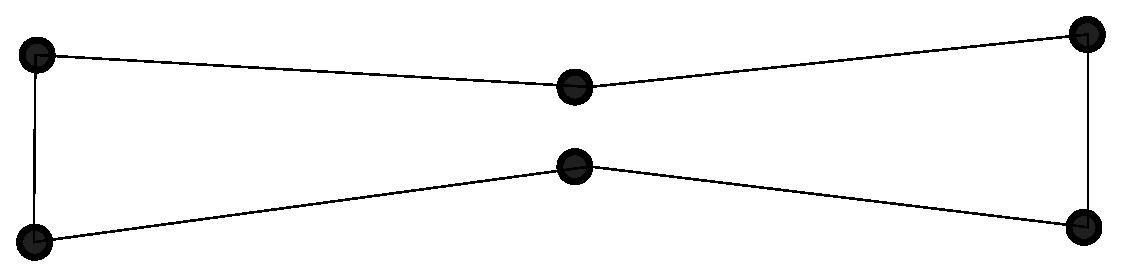
\includegraphics[width=6cm]{miscimages/closest-pair-example.eps}
       \caption{\label{fig:closestpair} Example where the segment joining the closest pair of points does not lie along the TSP tour}
     \end{figure}



     However, all attempts at constructing examples where the intersection with the 1-NNG is \textit{empty} failed. \footnote{Notice that \autoref{fig:closestpair} is not a counterexample!}And so did a
     literature search! The closest matching reference we found was \cite{hougardy2014edge} which \textit{eliminates} edges 
     that cannot be part of a Euclidean TSP tour on a given instance of points, based on checking a few simple, local geometric inequalities. \footnote{The author believes this will be a userful reference for future work}
     There was also a very much related discussion thread on David Eppstein's \href{https://www.ics.uci.edu/~eppstein/junkyard/dt-not-tsp.html}{webpage}. 
     A small counter-example to Michael Shamos' conjecutre from his unpublished notes --- that the TSP is a \textit{subgraph} of the Delaunay --- is given near the bottom of that link. 
     
     But the thread says nothing about whether the DT \textit{must} intersect the TSP at least a certain fraction of times, or indeed even once. \footnote{Perhaps, we can follow up with Dillencourt or Eppstein if they have notes on this?}

     See also this \href{https://web.colby.edu/thegeometricviewpoint/2015/03/09/delauney-triangulations-and-the-traveling-salesman/}{blogpost} on the topic, which 
     talks about using the Delaunay Triangulations for generating heuristically good (no bounds are given) TSP tours. Another approach using Del Tris
     is taken in \href{https://www.researchgate.net/publication/215753374_An_On_log_n_Heuristic_for_the_Euclidean_Traveling_Salesman_Problem}{this technical report} 

     Knowledge of some family of easily computed edges that are necessarily part of a TSP solution could potentially be used to speed up some 
     of the existing solutions to TSP using combinatorial optimization methods; see, e.g., Concorde \cite{applegate2009certification} and other papers of Bill Cook
     \footnote{The landmark PTAS'es for the TSP, such as those of Mitchell \cite{mitchell1999guillotine} and Arora\cite{arora1996polynomial},  are too complicated to be put into code (yes, even Python!). On the other hand, the Concorde library \cite{applegate2009certification} or Helsgaun's methods\cite{helsgaun2000effective}  use a whole kitchen-sink of practical techniques such as $k$-local swaps, branch-and-bound, branch-and-cut to generate  near-optimal (if not optimal) tours very fast. But it would be interesting to investigate the behavior of the various graphs with respect to the techniques used in the PTAS'es of Mitchell and Arora. Maybe we can augment them with the probabilistic method (the pigeon-hole principle on steroids!) or something from Ramsey Theory to prove the existence of an intersection??}.

     To spur our intuition,  we investigate the conjecture experimentally in this short report 
     \footnote{This report has been written as a literate program \cite{knuth1984literate,ramsey2008noweb} to weave together the code, documentations, explanations and generated data into the same document. Brickbats and bouqets on the author's preliminary stab at Literate Programming are most welcome.}
     using TSPLIB and Concorde in tandem. TSPLIB \cite{reinelt1991tsplib} is an online collection of medium to large scale instances of the Metric, the Euclidean and a few other variants of the TSP 
     Concorde can compute the optimal solutions in nearly all the instances; the certificate of optimality --- as always! --- coming from the comparsion of the computed tour-length against 
     a lower bounds (also computed by Concorde).

     For starters,  we investigate the following questions \footnote{Experimental answers to other questions will be barnacled onto the report as it grows}: 
     for each symmetric 2-D Euclidean TSP instance from TSPLIB for which we have an optimal solution, does

     \begin{itemize}
     \item $TSP \cap (k{\text -})NNG \stackrel{?}{=} \varnothing$, for $k=1,2,\ldots$
     \item $TSP \cap \; \text{Delaunay Graph} \stackrel{?}{=} \varnothing$
     \item For question 1 what fraction (a fourth?, a fifth?)of the $n$ edges of a TSP-tour share its edges with the  $k$-NNG does the TSP intersect for various values of $k$? 
     \item Are there any structural patterns observed in the intersections? Specifically, does \textit{at least } 
           one edge from the intersection with the $1$-NNG have one of its \textit{vertices} on the convex hull? 
           \footnote{This indeed seemed to be the case in all the author's failed attempts at a counter-example, and so a proof/disproof of this conjecture would be helpful}
           More generally, is this true for every layer of the onion, and not just the outer layer (i,e, the convex hull)?
     \end{itemize}

     See also the Appendix \autoref{sec:questions} for a running wishlist of questions that come out during discussions. 

     As an aid in constructing possible counter-examples, a GUI interface is provided to mouse-in points and then 
     run various tests on the points inputted. 
     
     If you don't have  Python 3.7+ on your machine, download the free  \href{https://www.anaconda.com/products/individual}{Anaconda} distro of Python; 
     it comes with most of the batteries included. See Appendix \autoref{sec:install} for instructions on how to install and run the code. 


\end{description}
